\section{Systematic parameter variation (1 page)}
\label{section:contribution_2}

{\color{red} Wie k\"onnen wir diesen Abschnitt sinnvoll strukturieren?}

In this work, we propose an component-based approach for the exploration and evaluation of future transportation scenarios. Transportation scenarios are considered with respect to the power grid and traffic network. The approach enables the formulation of transportation scenarios through different parameters. Scenarios are defined by objectives, situations and infrastructures representing the defining model parameters. An overview of this approach is shown in Figure~\ref{fig:approach}. 

\begin{figure}[h]
	\centering
	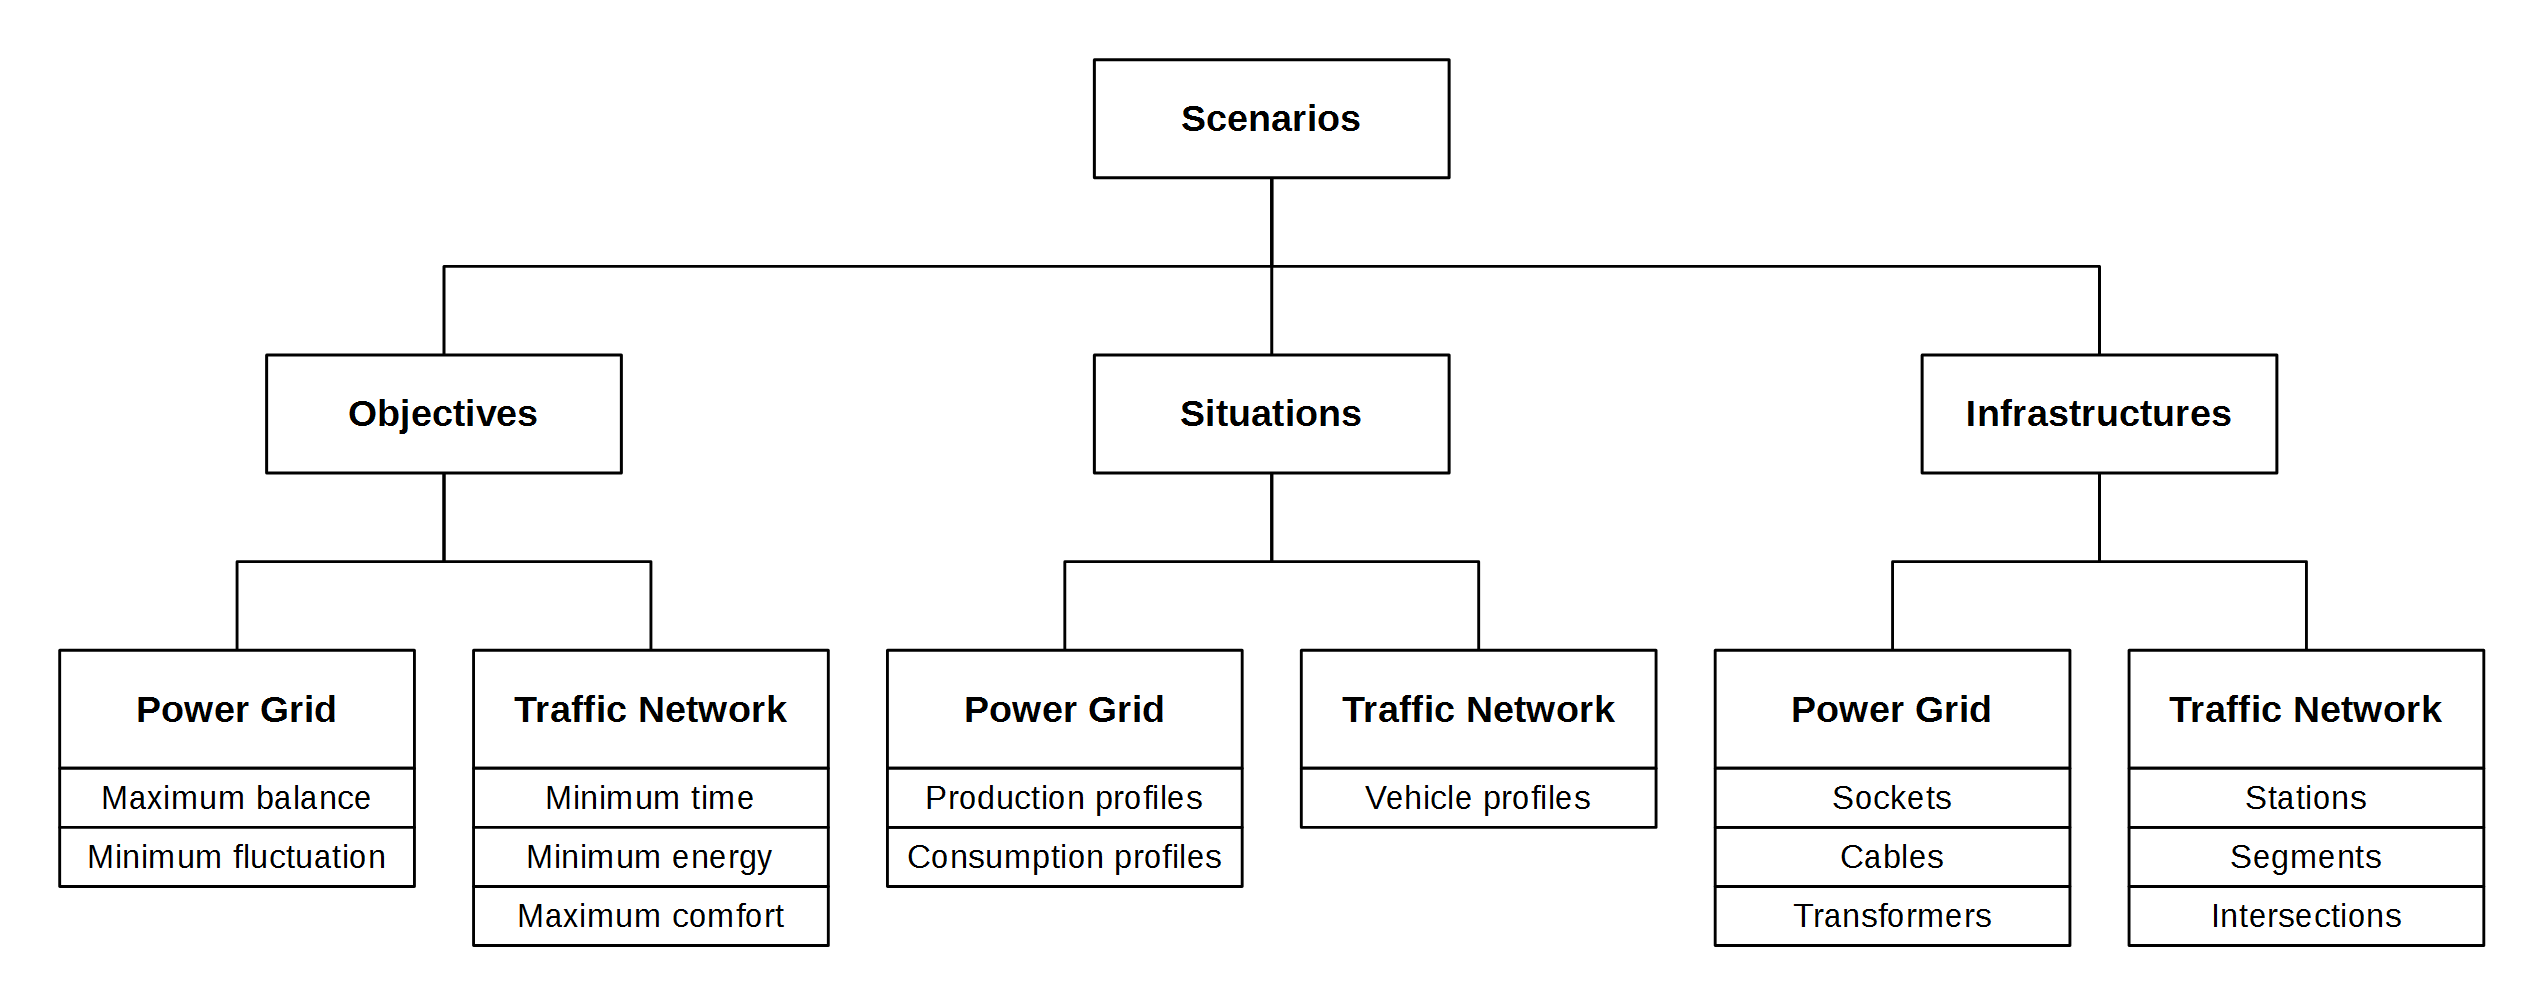
\includegraphics[width=\columnwidth]{../gfx/approach.png}
	\caption{Overview of transportation scenario modeling including objective, situation and infrastructure parameters for the power grid and the traffic network.}
	\label{fig:approach}
\end{figure}

\textit{Objectives} represent operational costs of different components, such as the traffic network and the power grid. 

\textit{Situations}  describe dynamic behavior such as profiles of individual traffic participants and loads on the power grid (i.e. production and consumption).

\textit{Infrastructures} represent the static structure and landscape of the contained power grid and traffic network. 

After scenario formulation, the approaches enables exploring and identifying the interactions between model parameters. We distinguish four types of parameter variation:

\subsubsection{Scenario variation}

\subsubsection{Objective variation}

\subsubsection{Situation variation}

\subsubsection{Infrastructure variation}